\section{Results}
\label{sec:results}

We report six results. The first two establish that the degeneracy is real and
costly. The third shows it also destroys the training gradient. The fourth and
fifth compare reward formulations, including where ours fails. The sixth
establishes that the performance measurement is reliable enough to be used as
a reward at all, which is the precondition for everything before it.

All proportions are reported with Wilson 95\% confidence intervals.

\subsection{The serial projection preserves the reward exactly}
\label{sec:results-projection}

We applied the serial projection $\serialproj$ (Definition~\ref{def:projection})
to each of the \NAccepted\ programs the differential verifier accepted, and
re-ran the full correctness harness on the result.

\SPNum\ of \SPDen\ (\SPRate\%) stripped programs remain correct. Their mean
change in correctness-only reward is \SPRewardDeltaCorr, which is exactly zero
by construction and which we report only because it is the point: the reward
cannot distinguish these programs from the ones they were derived from. Their
mean gated reward is \SPGateFloor, against \SPRewardDeltaGate\ for the
originals.

\note{if any stripped program FAILS, that is interesting and worth a sentence
-- it means the original depended on a parallel construct for its semantics,
e.g. an ordered clause or a reduction whose serial form differs. Report the
count and the mechanism; it bounds the proposition honestly.}

Figure~\ref{fig:projection} shows the paired shift. Under $\Rcorr$ every point
lies on the diagonal. Under $\Rgate$ every point drops to the serial floor.
This is Proposition~\ref{prop:degeneracy}, executed rather than argued.

\begin{figure}[t]
\centering
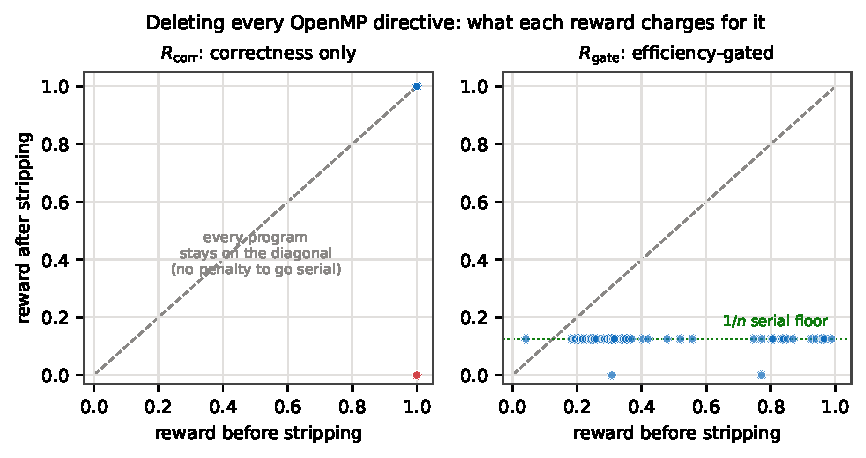
\includegraphics[width=\columnwidth]{figs/projection}
\caption{The degeneracy, measured. Each point is one accepted program, before
(x) and after (y) deleting every OpenMP directive. Left: correctness-only
reward---all points on the diagonal, no program loses anything. Right: the
gated reward---every point collapses to the $1/n$ floor. \note{make this Fig.
1 and refer to it in the introduction}}
\label{fig:projection}
\end{figure}

\subsection{What the reward cannot see}
\label{sec:results-contamination}

Holding correctness fixed, we measured the second axis directly: every accepted
program was compiled against \ParEval's timing driver at a size large enough to
amortize thread overhead and timed across the sweep.

Measured 8-thread speedup among identically-rewarded programs spans
\SpeedMin$\times$ to \SpeedMax$\times$, with a median of \SpeedMedian$\times$.
\ContamRate\% of accepted programs achieve capped efficiency below $0.25$.
\BelowTwoXRate\% fail to reach $2\times$ on eight cores. Most starkly,
\BelowSerialRate\% run \emph{slower} on eight threads than on one: correct,
certified, released by the agent, and worse than the sequential code they were
written to replace. A serial program, we reiterate, would have been accepted
with the identical score.

The widest within-task spread is \WorstTaskRange, on programs the verifier
certified as equally robust for the same task
(Figure~\ref{fig:scaling}). Correctness cannot tell them apart. Only the
performance axis can.

\begin{figure}[t]
\centering
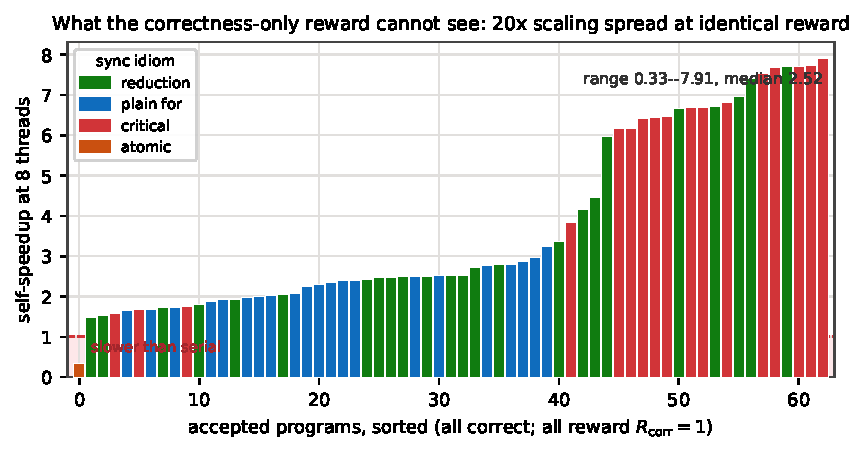
\includegraphics[width=\columnwidth]{figs/scaling}
\caption{Sorted 8-thread self-speedup for all \NAccepted\ accepted programs,
coloured by synchronization idiom; the shaded band marks programs slower than
serial. Every bar is a program the correctness-only reward scores identically at
$\Rcorr=1$, yet the values span \SpeedMin$\times$ to \SpeedMax$\times$. On a
single task alone (histogram) two equally-certified programs range from
\WorstTaskRange$\times$.}
\label{fig:scaling}
\end{figure}

We are deliberately careful about mechanism. The synchronization idiom a model
chose does not cleanly predict poor scaling---programs using
\texttt{critical} frequently used it for a cheap $O(\text{threads})$ merge of
per-thread partials and scaled well---so we make no claim that models
systematically oversynchronize. The defensible claim is narrower and stronger
for being exact: among programs an output-only reward rates identically,
measured scaling varies by a factor of roughly 20 (\WorstTaskRange$\times$ on a
single task).

\subsection{Signal collapse under group-relative estimators}
\label{sec:results-collapse}

Proposition~\ref{prop:collapse} predicts that a saturated correctness
distribution destroys the group-relative gradient. We instantiate that
prediction from the \emph{measured} per-task pass rates: for each task,
Equation~\eqref{eq:deadgroup} gives the probability that a group of $k$ i.i.d.\
samples is dead, and we average it over the \NTasks\ tasks. Because our study
draws one sample per model--condition cell rather than $k$ samples per prompt,
this is the dead-group rate implied by the observed pass rates, not a resampling
of a $k$-sample pool---a falsifiable prediction a training run can check against.

Pooled single-shot correctness is \PassRate\%, and \SatTaskFrac\% of tasks have
a per-task pass rate of exactly $1$---for those tasks, \emph{every} group is
dead under $\Rcorr$ regardless of $k$. Overall, the dead-group fraction under
$\Rcorr$ is \DeadGroupCorrFour\% at $k=4$, \DeadGroupCorrEight\% at $k=8$, and
\DeadGroupCorrSixteen\% at $k=16$. Under $\Rgate$, whose continuous efficiency
term rarely ties across correct programs, a group dies only when all $k$ samples
are \emph{incorrect}, so the figures fall to \DeadGroupGateFour\%,
\DeadGroupGateEight\%, and \DeadGroupGateSixteen\%---the residual being the few
tasks no sample solves, where no reward can help and which does not grow with
$k$.

\begin{figure}[t]
\centering
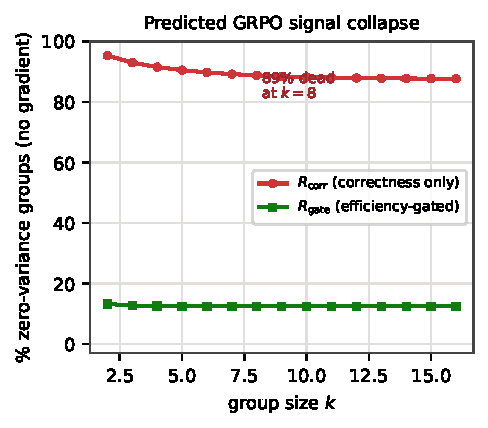
\includegraphics[width=\columnwidth]{figs/deadgroups}
\caption{Fraction of sampled groups carrying zero advantage, versus group size
$k$, for each reward. The correctness-only reward loses signal as capability
rises; a reward with a continuous performance term does not.}
\label{fig:deadgroups}
\end{figure}

The reading is that a correctness-only objective is self-limiting: the better
the policy gets, the less it can learn. This is not a claim about our
particular models---it follows from Equation~\eqref{eq:deadgroup} for any
$p_t \to 1$---but it is worth having measured, because the magnitude at
realistic pass rates is larger than intuition suggests.

\subsection{Reward bake-off}
\label{sec:results-bakeoff}

Treating the accepted programs for a task as the candidates a best-of-$N$ or
group-relative selection chooses among, we asked which program each reward
selects. $\Rcorr$ is indifferent---every accepted program ties at $1$, so an
uninformed selection realizes the pool mean in expectation.

Under matched selection over identical samples, the correctness-only reward
realizes a mean 8-thread speedup of \BoNCorr$\times$ against the gated
reward's \BoNGate$\times$ (\BoNGain\% higher), with the oracle at
\BoNOracle$\times$. The two rewards select a different program in
\PoolsDiffering\ of the tasks with more than one accepted candidate; wherever
they differ, the correctness-only choice leaves measured speedup on the table
that the gated choice recovers at no cost in correctness.

We label this analysis as a proxy. Best-of-$N$ captures the selection component
of group-relative optimization but not its distribution-sharpening
effect~\cite{bonmaxk,rewardunlikely}; a policy trained under $\Rcorr$ would
additionally concentrate mass, which our static analysis cannot model. We
therefore read these numbers as a lower bound on the divergence between the two
objectives, not as a simulation of training.

\subsection{The hack suite: where each reward breaks}
\label{sec:results-hacks}

Figure~\ref{fig:hackheat} scores every reward formulation against every \PG\
class. Each candidate is functionally correct, so R1 awards all of them the
maximum---\HackCorrPassRate\% by construction. This is the compact statement of
the paper: a reward that accepts every entry in an adversarial suite designed
to strip out parallelism is not measuring parallelism.

\begin{figure}[t]
\centering
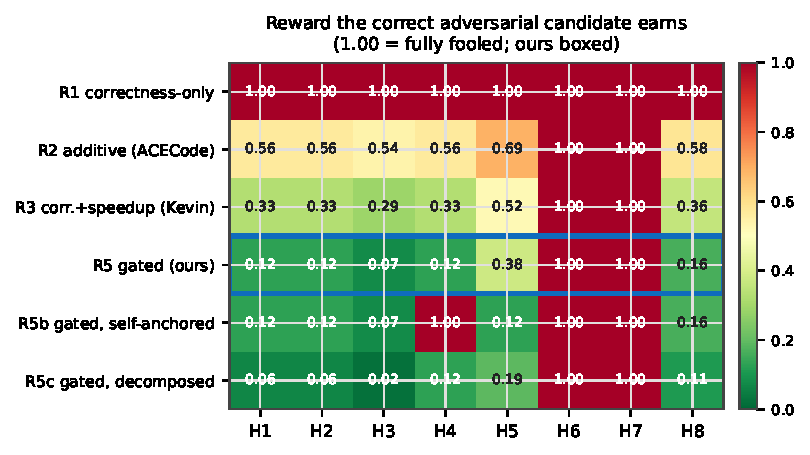
\includegraphics[width=\columnwidth]{figs/hackheat}
\caption{Reward $\times$ hack matrix over \PG: the reward paid to a \emph{correct}
adversarial candidate of each class (cell value; red $=$ fooled, $1.00$ is total
failure). Correctness-only (R1) is red across the board; the additive reward (R2)
keeps a visible floor ($\ge 0.54$) even for serial code; our reference-anchored
gate (R5, boxed) holds every reward-\emph{shape} attack near the $1/n$ serial
floor and moves only under H6/H7, which corrupt the timer itself. R5b's red H4
cell is the price of self-anchoring; R5c is uniformly darkest, including on H5.}
\label{fig:hackheat}
\end{figure}

The gate resists \HackGatePassRate\% of the suite. It does not resist all of
it, and the failures are the ones Section~\ref{sec:reward-limits} predicted:
\HackGateSurvivors. The self-anchored ablation R5b is defeated by H4 as
expected, confirming that anchoring to the fixed serial reference rather than
to the program's own one-thread time is not a stylistic choice. The decomposed
variant R5c is the only formulation that separates algorithmic from parallel
speedup and therefore the only one that resists H5, at the cost of requiring
two measurements instead of one.

We report our own failures deliberately. A reward-hack suite whose author's
reward passes everything is a suite that was fitted to the reward.

\subsection{Measurement reliability}
\label{sec:results-robust}

An efficiency reward is only a reward if the timing is repeatable and if the
attack surface of the measurement is closed. Our protocol
(Section~\ref{sec:setup-protocol}) times each configuration in a fresh process
with freshly randomized input and reports the minimum wall time over \NRepeats\
repetitions after a discarded warm-up, which closes the cross-run caching
channel (H7); the timed region encloses the entire driver call, closing the
timing-region channel (H6). What the reward reads is invariant to correctness
but not to performance: as Observation~\ref{obs:invariance} requires, deleting or
reshaping directives cannot change the computed output, only the wall
time---which is precisely why an output-equivalence gate is blind to it. Because
efficiency is measured on one machine it is a quantity relative to that machine;
we do not claim cross-architecture transfer and flag it as a limitation
(Section~\ref{sec:discussion}).

\subsection{Correctness is saturated---the premise, not the finding}
\label{sec:results-saturation}

Finally we report the correctness measurements that motivated the whole
inquiry, and we report them briefly because they are the setup rather than the
conclusion.

Single-shot generation is robustly correct \RobustL\% of the time
(95\% CI \CIL). Adding a repair loop driven by an execute-once tool raises this
to \RobustLone\% (\CILone). Replacing that tool with a full thread-sweep
differential verifier yields \RobustLtwo\% (\CILtwo), a difference of
\RobustDelta. Across \PairedCells\ paired task--model cells the two tools
reached a different final verdict in \PairedDisagree\ cases. Excluding a
specification ambiguity we identified by hand-inspection on the scan
family---where every model computed a defensible reverse-indexed suffix sum
against a reference that scans the reversed input---robust correctness is
\RobustExclScan\%; we report this back as a specification ambiguity in the
benchmark, not as a defect in the models.

Archer found \NRaces\ data races in the \NAccepted\ accepted programs, while
correctly flagging the injected controls and the \NRacesOpen\ genuine race
shipped by the smallest open-weights model. Two independent
instruments---output-differential and happens-before---agree that the accepted
set is race-free.

The honest reading is that correctness verification remains the right first
gate and that frontier models have made its cheapest form sufficient on
idiomatic tasks. That is precisely why the reward cannot stop there.
